% [原文 p.83]
其中，求和遍历给 $N$ 的各成分赋 level $k$ 最高权的全部映射 $\mu:\{1,\dots,m\}\to P_+(k)$。

\section{映射类群的射影表示与拓扑场论}
\takeaway{以 Witten 不变量为原料，用 $(2g,2g)$ tangle 的 tangle 算子拼出映射类群 $\cM_g$ 在共形块空间 $V_\Sigma$ 上的射影表示 $\rho$，其 2-余循环由符号差之差给出；再用 Heegaard 分解把 $\rho$ 与 $Z_k(M)$ 联系起来，得到 2+1 维拓扑场论的例子。}

前节构造的三维流形 Witten 不变量 $Z_k(M)$，用到了 Dehn 手术这一三维流形的表示。其实，把理论的框架稍加推广，就能说明可以构造出 Atiyah 意义下的 2+1 维拓扑场论（topological quantum field theory）的例子。先一般地列出 Atiyah 意义下 $d+1$ 维拓扑场论的公理。

$d+1$ 维拓扑场论是指具有下述性质的函子 $Z$。

（1）对紧致、无边界、带定向的 $d$ 维微分流形 $\Sigma$，对应一个有限维复线性空间 $Z_\Sigma$。
（2）对紧致、带定向的 $d+1$ 维微分流形 $Y$，若 $\partial Y=\Sigma$，则确定一个向量 $Z(Y)\in Z_\Sigma$。

进而要求 $Z$ 满足以下性质 (A1)--(A5)。

（A1）把 $\Sigma$ 的定向反转所得的流形记作 $-\Sigma$，则 $Z_{-\Sigma}=Z_\Sigma^*$ 成立。这里，$Z_\Sigma^*$ 是 $Z_\Sigma$ 作为 $\C$ 上线性空间的对偶空间。

（A2）对不相交的并集 $\Sigma_1\sqcup\Sigma_2$，有 $Z_{\Sigma_1\sqcup\Sigma_2}=Z_{\Sigma_1}\otimes Z_{\Sigma_2}$ 成立。

由上面的 (A1) 与 (A2)，对满足 $\partial Y=(-\Sigma_1)\sqcup\Sigma_2$ 的紧致、带定向的 $d+1$ 维微分流形 $Y$，确定一个线性映射 $Z(Y)\in\Hom_\C(Z_{\Sigma_1},Z_{\Sigma_2})$。这样的 $Y$ 称为 $\Sigma_1$ 与 $\Sigma_2$ 之间的配边（cobordism）。

（A3）对配边的合成 $\partial Y_1=(-\Sigma_1)\sqcup\Sigma_2$、$\partial Y_2=(-\Sigma_2)\sqcup\Sigma_3$，有
\[
  Z(Y_1\cup Y_2)=Z(Y_2)Z(Y_1)
\]
成立。

% [Tutor Note: (A1)、(A2) 决定了“边界反定向”与“不交并”的处理，由此才有 $Z(Y)\in\Hom_\C(Z_{\Sigma_1},Z_{\Sigma_2})$：若把 $\partial Y=(-\Sigma_1)\sqcup\Sigma_2$ 误写成 $\Sigma_1\sqcup\Sigma_2$，映射的方向就会反过来。]

% [原文 p.84]
（A4）$Z(\varnothing)=\C$ 成立。

（A5）设 $I$ 为单位区间，则 $Z(\Sigma\times I)$ 作为 $Z_\Sigma$ 的线性变换是恒等映射。

$Z$ 可以看作从“紧致、无边界、带定向的 $d$ 维微分流形及其间的配边”这一范畴，到“复线性空间及其间的线性映射”这一范畴的函子。下面叙述公理的几个推论。由 (A3) 与 (A5) 可知，$\Sigma$ 的保向微分同胚全体构成的群 $\Diff^+(\Sigma)$ 线性地作用于 $Z_\Sigma$。特别地，$Y$ 为无边界流形时，$Z(Y)$ 作为复数确定。这也可以如下求得：把 $Y$ 沿 $d$ 维流形 $\Sigma$ 切开，分解为两个带边流形 $Y_+$、$Y_-$ 的并集，使 $\partial Y_+=\Sigma=-\partial Y_-$，则确定 $Z(Y_+)\in Z_\Sigma$、$Z(Y_-)\in Z_\Sigma^*$，而 $Z(Y)$ 由 $Z_\Sigma$ 与 $Z_\Sigma^*$ 的自然配对给出：
\[
  Z(Y)=\langle Z(Y_+),Z(Y_-)\rangle.
\]
由 (A3)，这与分解方式无关，唯一确定。对 $f\in\Diff^+(\Sigma)$，把 $\Sigma\times I$ 的边界 $\Sigma\times\{0\}$ 与 $\Sigma\times\{1\}$ 粘合所得的流形记作 $\Sigma_f$，则用 $f$ 在 $Z_\Sigma$ 上的作用 $\rho(f)$，得 $Z(\Sigma_f)=\Tr\rho(f)$。特别地，取 $f$ 为恒等映射，可知
\[
  \dim Z_\Sigma=Z(\Sigma\times S^1).
\]
% [Tutor Note: 取下 $f=\id$ 时 $\rho(f)$ 是恒等映射，取迹即得 $\dim Z_\Sigma$；这正是二维拓扑场论里“配分函数等于态空间维数”的来源，也说明 $Z(\Sigma\times S^1)$ 必须按无边界情形解释。]

本节的目标是说明：把共形场理论的和乐取迹所构成的 Jones--Witten 理论，在 $d=2$ 的情形下是拓扑场论的一例。不过，上面的 Atiyah 公理只是大致的框架，实际理论中需要作若干修正。特别地，$\Diff^+(\Sigma)$ 的作用不是线性表示而是射影表示，这一点很重要，后面将详细解说。

§2.2 已说明：以 $n$ 个 $S^1$ 为边界、亏格为 $0$ 的曲面的映射类群 $\cM_{0,n}$ 线性地作用于共形块空间。这里把这个方法推广，构造一般亏格曲面的映射类群的表示。设 $\Sigma$ 为亏格 $g$ 的
% [原文 p.85]
带定向闭曲面。对 $\Sigma$ 的保向微分同胚全体 $\Diff^+(\Sigma)$ 的元素 $h,h'$，用“$h$ 与 $h'$ 彼此同痕”定义等价关系 $h\sim h'$，把按此等价关系分类所得的集合 $\Diff^+(\Sigma)/\sim$ 记作 $\cM_g$。$\cM_g$ 关于微分同胚的合成构成群，称之为 $\Sigma$ 的映射类群（mapping class group）。

对亏格 $g$ 的闭曲面 $\Sigma$，如下构造复线性空间 $V_\Sigma$。基本想法是：把 $\Sigma$ 实现为柄体 $H$ 的边界，再如图2.22 所示，用柄体中以二维圆盘为边界的闭曲线 $C_1,\dots,C_g$ 把曲面 $\Sigma$ 切开，从而使用 §2.2 所述的亏格 $0$ 情形的构造。本节也只讨论 $\fg=\fsl_2(\C)$ 的情形。

\begin{figure}[htbp]
  \centering
  
\includegraphics[width=0.72\textwidth]{figures/fig2.22.png}
  \figtitle{2.22}{亏格 $g$ 的闭曲面沿曲线 $C_1,\dots,C_g$ 切开。（原书 p.85）}
\end{figure}

在复平面的实轴上取 $2g$ 个点 $p_1,p_2,\dots,p_{2g-1},p_{2g}$，使其坐标满足 $0<z_1<z_2<\cdots<z_{2g-1}<z_{2g}$。固定正整数 $k$，给这些点对应仿射 Lie 代数 $\hat\fg$ 的 level $k$ 最高权 $\mu_1,\mu_1^*,\dots,\mu_g,\mu_g^*$。与 §2.2 一样，$\lambda^*$ 表示对应 $\cH_\lambda$ 的对偶表示 $\cH_\lambda^*$。此外，在原点对应 $\cH_0$，在无穷远点对应其对偶表示 $\cH_0^*$。对此定义的共形块空间，如 §1.4 所示，可以自然地嵌入不变张量空间
\[
  \Hom_{\fg}(V_{\mu_1}\otimes V_{\mu_1}^*\otimes\cdots\otimes V_{\mu_g}\otimes V_{\mu_g}^*,\C)
\]
之中。把这个嵌入下共形块空间的像记作 $V_{\mu_1\mu_1^*\cdots\mu_g\mu_g^*}$，并令
\[
  V_\Sigma=\bigoplus_{\mu_1,\mu_1^*,\dots,\mu_g,\mu_g^*\in P_+(k)}V_{\mu_1\mu_1^*\cdots\mu_g\mu_g^*}.
\]
% [Tutor Note: $V_\Sigma$ 是所有允许权对应的 $V_{\mu_1\mu_1^*\cdots\mu_g\mu_g^*}$ 的直和，不是其中某一项；下标中 $\mu_i$ 与 $\mu_i^*$ 成对出现，正对应图 $\Gamma$ 的两端各一个边界点。]

% [原文 p.86]
这里，$P_+(k)$ 是 level $k$ 的最高权集合；最高权用整数表示时 $P_+(k)=\{0,1,\dots,k\}$。$V_\Sigma$ 的基底如图2.23 所示，用这样的图 $\Gamma$ 表示：各边上赋 level $k$ 的最高权，围绕各顶点所汇集各边对应的权满足命题 1.15 所述 level $k$ 的 Clebsch--Gordan 条件。曲面 $\Sigma$ 实现为 $\R^3$ 中 $\Gamma$ 的正则邻域的边界。

映射类群中对应“沿某闭曲线 $C$ 把曲面切开、扭 $2\pi$ 后重新粘合”这一操作的微分同胚，如图2.24 所示，称为沿 $C$ 的 Dehn 扭转（Dehn twist），其同痕类记作 $\tau_C$。据 Lickorish，映射类群 $\cM_g$ 由沿图2.24 所示 $3g-1$ 条曲线 $\alpha_i,\beta_i$（$1\le i\le g$）、$\delta_j$（$2\le j\le g$）的 Dehn 扭转生成。

用 Verlinde 等式（命题 1.22），算得
\[
  \dim V_\Sigma=\sum_{\lambda\in P_+(k)}\Bigl(\frac{1}{S_{0\lambda}}\Bigr)^{2g-2}.
\]

下面说明：把前节所述的 Witten 不变量构造推广到带边三维流形，即可定义映射类群 $\cM_g$ 在 $V_\Sigma$ 上的作用。为此先作如下准备。首先如图2.23 所示，在 $\R^2\times I$ 内分别配置由亏格 $g$ 的闭曲面按上述方式构成的图 $\Gamma_1$、$\Gamma_2$。把 $\Gamma_1$、$\Gamma_2$ 的正则邻域所得的柄体分别记作 $H_1$、$H_2$。对映射类群 $\cM_g$ 的元素 $h$，把 $H_1$ 与 $-H_2$ 按 $h:\partial H_1\to\partial H_2$ 粘合所得的三维流形记作 $M$。又把 $\R^2\times I$ 看作 $\R^3\cup\{\infty\}$ 的子集，在 $\R^2\times I$ 内取一条与 $\Gamma_1$、$\Gamma_2$ 不相交的带 framing 的链环 $L$，使得 $M$ 可由沿 $L$ 的 Dehn 手术得到。具体地，把 $h$ 表为 Lickorish 生成元的乘积，对每个 Dehn 扭转按图2.24 下方那样对应一个 $(2g,2g)$ tangle。再把 Dehn 扭转的乘积对应为 tangle 的合成，所得的链环记作 $L(h)$。

把图 $\Gamma_1$、$\Gamma_2$ 以及带 framing 的链环 $L(h)$ 合在一起，
% [原文 p.87]
看作 §2.2 所定义意义的 $(2g,2g)$ tangle。这个 tangle 记作 $T$。给链环 $L(h)$ 定向，并按图2.23 那样赋权 $\mu_1,\dots,\mu_g,\nu_1,\dots,\nu_g$。于是，对给链环 $L(h)$ 各成分赋权 $\lambda:\{1,2,\dots,m\}\to P_+(k)$ 的每一种方式，按 §2.2 的构造，作为 tangle 算子得到线性映射
\[
  J(T;\lambda)_{\mu\nu}:V_{\mu_1\mu_1^*\cdots\mu_g\mu_g^*}\longrightarrow V_{\nu_1\nu_1^*\cdots\nu_g\nu_g^*}.
\]
利用它，令
\begin{align*}
  \rho(h)_{\mu\nu}
  &=\sqrt{S_{0\mu_1}\cdots S_{0\mu_g}}\,\sqrt{S_{0\nu_1}\cdots S_{0\nu_g}}\\
  &\quad\times C^{\sigma(L(h))}\sum_{\lambda}S_{0,\lambda(1)}\cdots S_{0,\lambda(m)}J(T;\lambda)_{\mu\nu}.
\end{align*}
记号与前节 Witten 不变量的定义相同。这样对 $\lambda$ 求和之后，所得结果与链环定向的选取无关。进而，用 $\rho(h)=\bigoplus_{\mu\nu}\rho(h)_{\mu\nu}$ 定义
\[
  \rho(h):V_\Sigma\longrightarrow V_\Sigma.
\]
如此便得到映射 $\rho:\cM_g\to GL(V_\Sigma)$。与前一节证明 Witten 不变量在 Kirby 操作下不变的论证一样，可知 $\rho(h)$ 不依赖于把 $h$ 表为 Lickorish 生成元乘积的方式，而由 $h\in\cM_g$ 确定。

\begin{figure}[htbp]
  \centering
  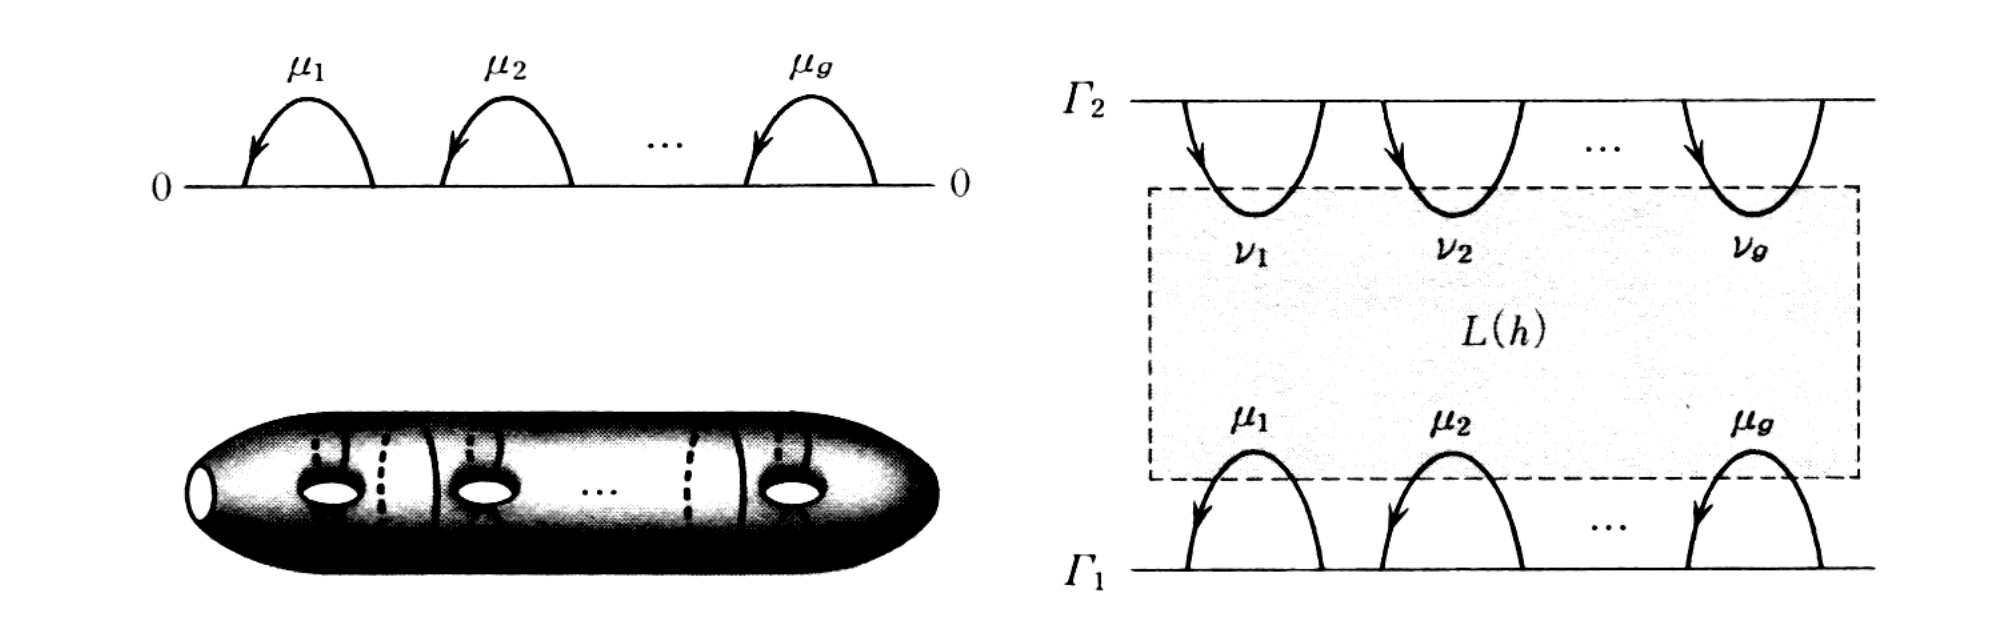
\includegraphics[width=0.96\textwidth]{figures/fig2.23.png}
  \figtitle{2.23}{图的正则邻域的边界所表示的曲面，分解为三个带洞球面之和。（原书 p.87）}
\end{figure}

对映射类群 $\cM_g$ 的元素 $x,y$，按上述方式对应 $(2g,2g)$ tangle $T(x)$、$T(y)$、$T(xy)$，对其中分别出现的链环 $L(x)$、$L(y)$、$L(xy)$，令
% [原文 p.88]
\[
  \xi(x,y)=C^{\sigma(xy)-\sigma(x)-\sigma(y)}.
\]
由以上讨论，可得下述命题。

\begin{proposition}{2.19}
  上面定义的 $\rho:\cM_g\to GL(V_\Sigma)$ 满足
  \[
    \rho(xy)=\xi(x,y)\rho(x)\rho(y).
  \]
  也就是说，$\rho$ 是关于 2-余循环 $\xi$ 的射影表示。
\end{proposition}

% [Tutor Note: 把 $h$ 换一种 Lickorish 生成元的分解方式时，$\rho(h)$ 只会相差一个标量，这个标量正是 $\xi$；因此 $\rho$ 是射影表示而不是线性表示，不能直接当成群同态使用。]

\begin{figure}[htbp]
  \centering
  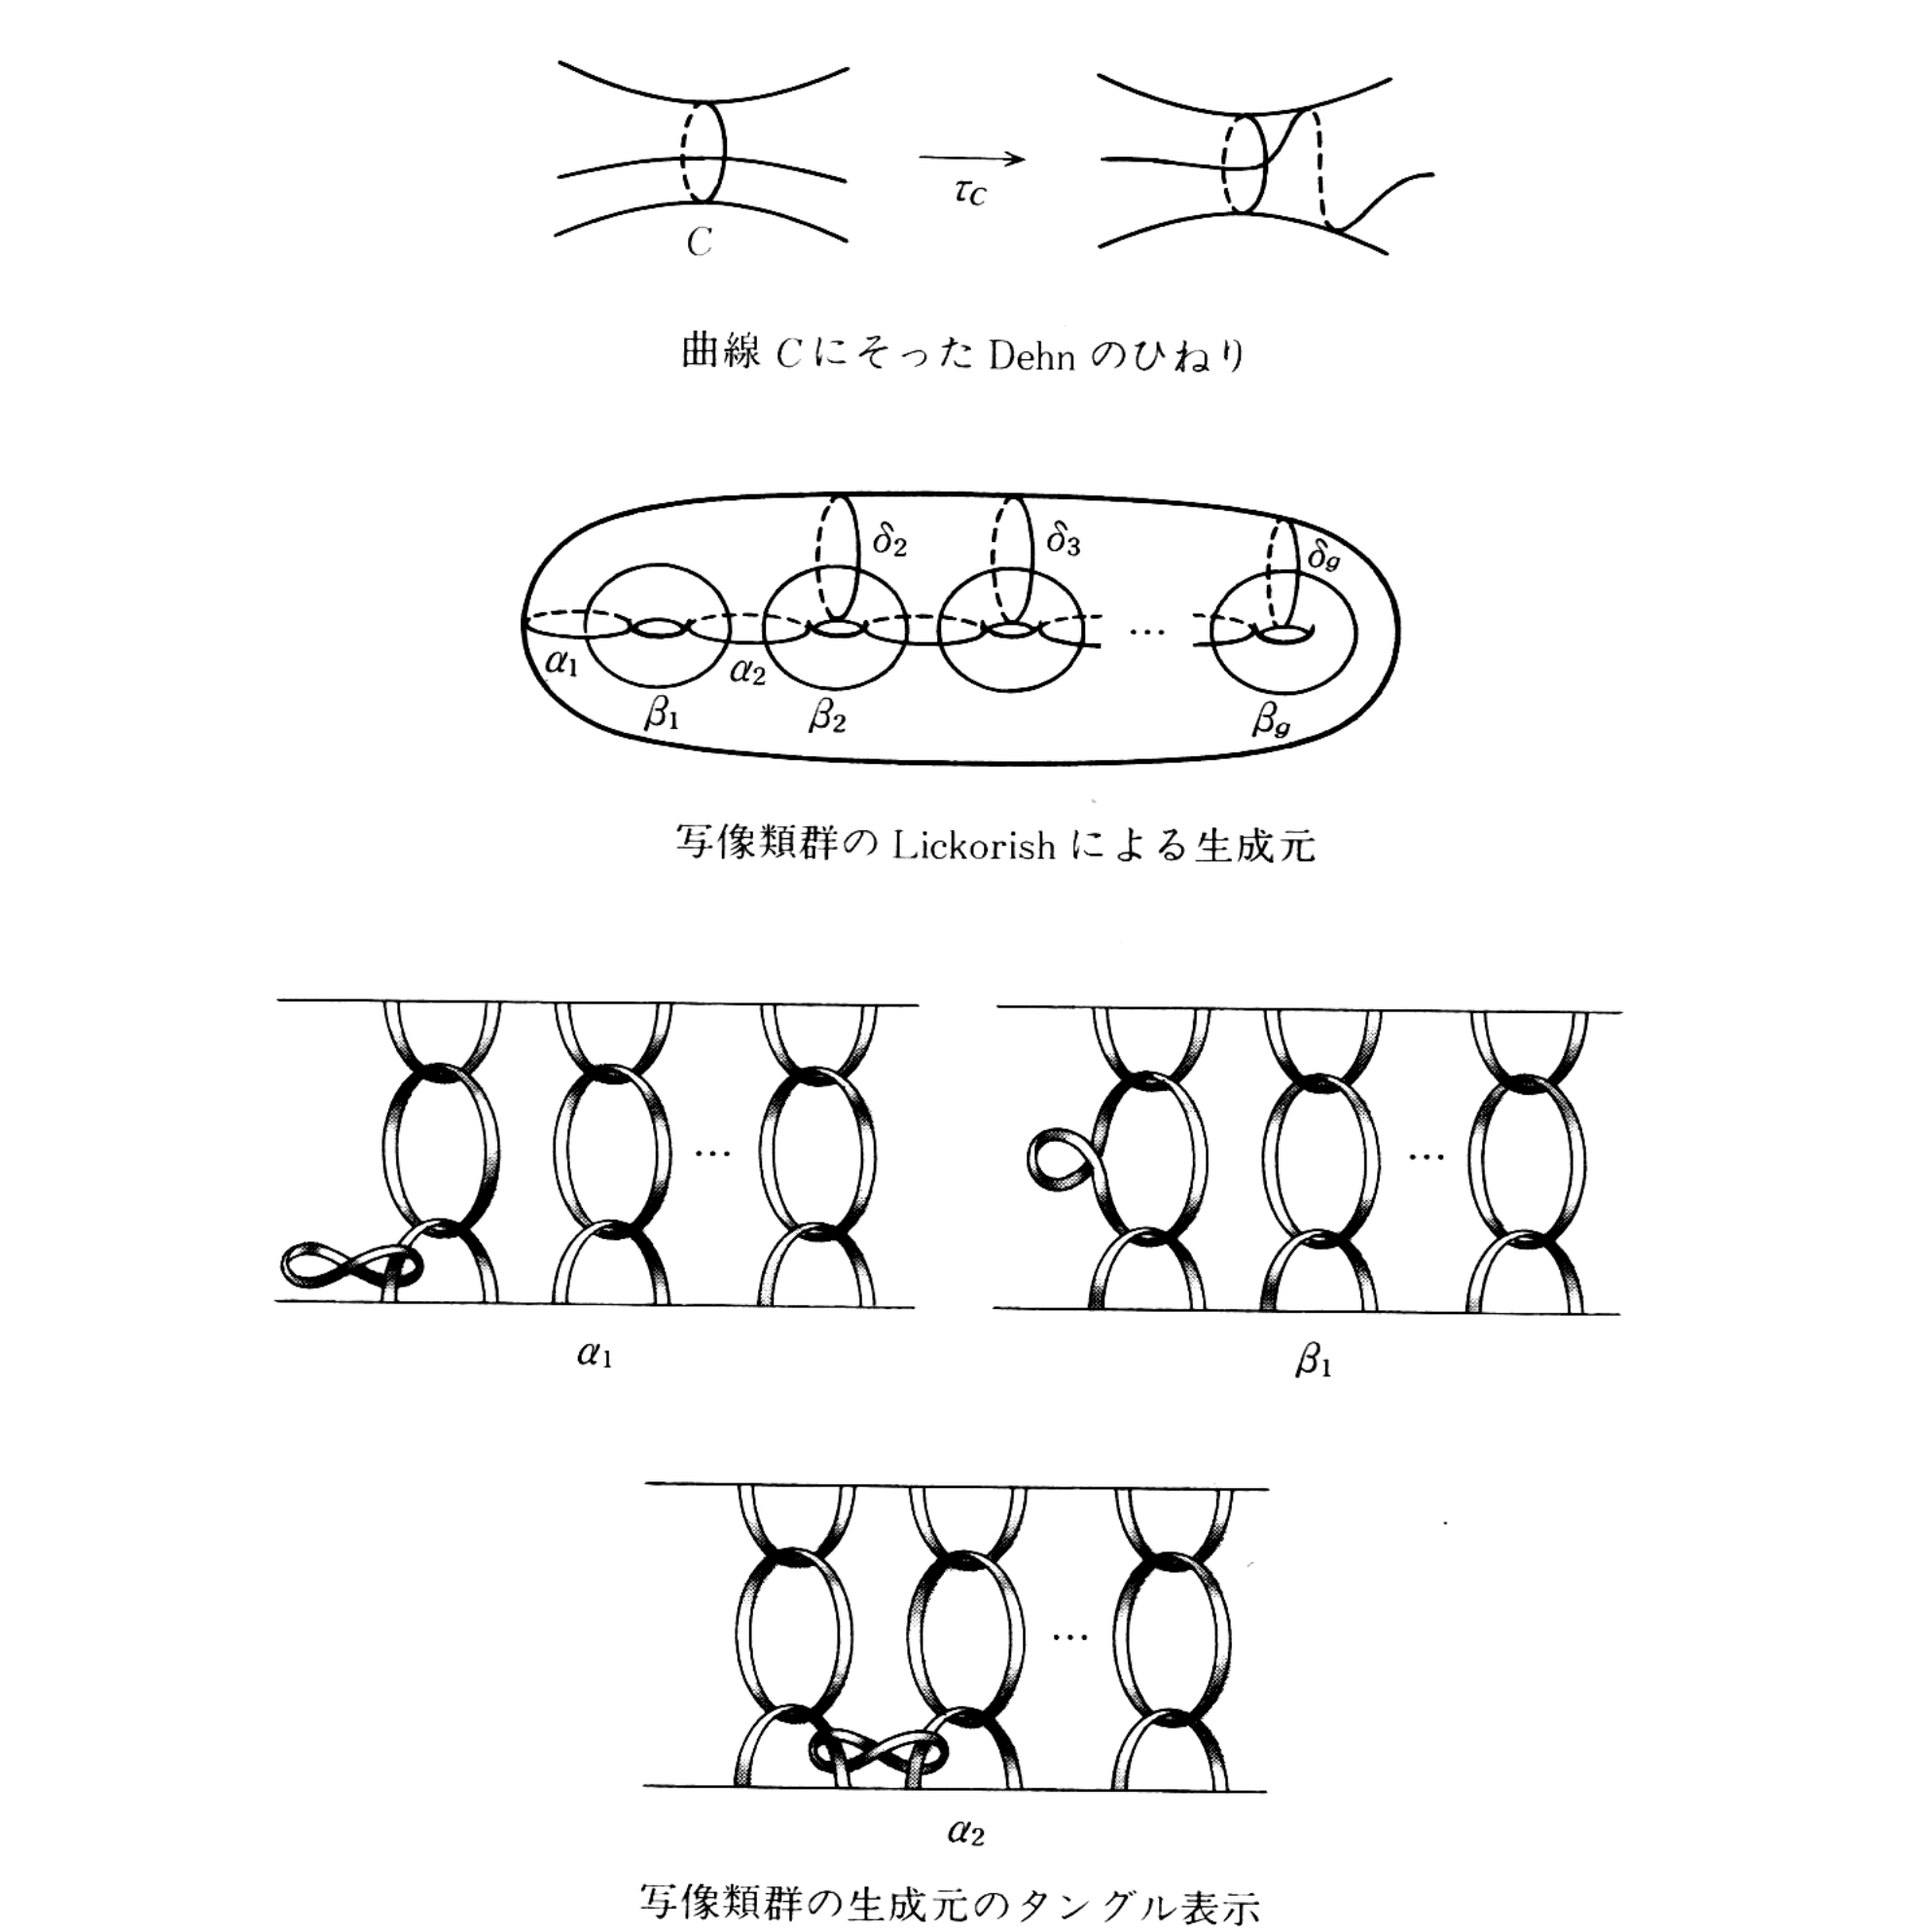
\includegraphics[width=0.90\textwidth]{figures/fig2.24.png}
  \figtitle{2.24}{原书无图注（原书 p.88）}
\end{figure}

% [原文 p.89]
这里，$\xi$ 是取值于 $\C^*$ 的 $\cM_g$ 的 2-余循环。即 $\xi$ 满足
\[
  \xi(xy,z)\xi(x,y)=\xi(x,yz)\xi(y,z).
\]
这由 $\rho((xy)z)=\rho(x(yz))$ 立即得到。

$g=1$ 时，映射类群 $\cM_1$ 同构于 $SL_2(\Z)$。此时，把给边赋权 $\lambda$ 的图 $\Gamma$ 对应的 $V_\Sigma$ 的基底记作 $v_\lambda$，则关于这组基底，$SL_2(\Z)$ 的生成元 $S$、$T$ 的作用分别用 $S_{\lambda\mu}$ 与 $\Delta_\lambda$ 表为
\begin{equation}
  Sv_\lambda=\sum_{\mu}S_{\lambda\mu}v_\mu \tag{2.28}
\end{equation}
\begin{equation}
  Tv_\lambda=\exp(2\pi\sqrt{-1}\,\Delta_\lambda)v_\lambda \tag{2.29}
\end{equation}
事实上，关于变换 $S$ 的结果来自 §2.3 所述 Hopf 链环的命题 2.15；关于变换 $T$ 的结果来自 §2.2 所述链环 framing 的命题 2.6。把它与用 Verlinde 基底描述 $SL_2(\Z)$ 在环面共形块空间上的作用相比较，可见除 $C$ 的幂次不同外，两者一致。

下面看命题 2.19 的映射类群射影表示的几条性质。关于 $V_\Sigma$，如 §2.1 所述，反复施行图2.2 的操作，可以给出对应于另一张图的基底。这些基底之间的变换矩阵由 KZ 方程的连接矩阵给出。如图2.23 那样把柄体实现为图的正则邻域，并把闭曲面看作其边界，则关于与图的边 $e$ 横截相交的二维圆盘的边界 $C(e)$，其 Dehn 扭转在该基底下对角化。$C(e)$ 的特征值用边 $e$ 上赋予的权 $\lambda(e)$ 表为 $\exp(-2\pi\sqrt{-1}\,\Delta_{\lambda(e)})$。例如，对图2.23 所示的基底，$\alpha_1,\delta_2,\cdots,\delta_g$ 的作用已对角化。
% [Tutor Note: 式 (2.28) 中的 $S$ 既是 $SL_2(\Z)$ 的生成元，又是 $S$ 矩阵的来源，两者记号相同但含义不同；指标顺序为 $S v_\lambda=\sum_\mu S_{\lambda\mu}v_\mu$，其中行指标是 $\lambda$，列指标是 $\mu$。]

下面说明这里构造的映射类群射影表示与三维流形 Witten 不变量的关系。一般地，设 $M$ 为紧致、无边界、带定向的三
% [原文 p.90]
维流形。众所周知，$M$ 可用某个亏格的柄体 $H_g$ 表为 $M=H_g\cup_h(-H_g)$。这里，$h\in\cM_g$ 是粘合 $H_g$ 边界的映射 $h:\partial H_g\to\partial H_g$。这样的三维流形分解称为 Heegaard 分解（Heegaard splitting）。Heegaard 分解的存在性可如下证明：取三维流形的单纯剖分及其对偶剖分，对两者分别取由 $0$-单形与 $1$-单形组成的子复形的正则邻域。利用 Heegaard 分解，$Z_k(M)$ 可表示如下。首先，在图2.23 的图所表示的 $V_\Sigma$ 的基底中，把对应“所有边都赋权 $0$”的图的向量记作 $v_0$。下述命题成立。

\begin{proposition}{2.20}
  设 $M=H_g\cup_h(-H_g)$ 为 Heegaard 分解，则 $M$ 的 Witten 不变量用命题 2.19 的射影表示 $\rho$ 表为
  \[
    Z_k(M)=S_{00}^{-g+1}\langle v_0^*,\rho(h)v_0\rangle.
  \]
  这里，$v_0^*$ 是 $v_0$ 的对偶基底，$\langle\,,\rangle$ 是 $V_\Sigma$ 与其对偶空间之间的自然配对。
\end{proposition}

对映射类群 $\cM_g$ 的元素 $h$，如图2.25 所示，给柄体 $H_g$ 添加一个 1-柄得到 $H_{g+1}$，并用把曲线 $\alpha$ 移到 $\beta$ 的微分同胚，把 $h$ 在同痕意义下扩充为 $\partial H_{g+1}$ 的微分同胚，所得 $\cM_{g+1}$ 的元素记作 $\tilde h$。由 Heegaard 分解 $H_{g+1}\cup_{\tilde h}(-H_{g+1})$ 给出的三维流形，是把 $M=H_g\cup_h(-H_g)$ 与 $S^3$ 作连通和所得流形，与 $M$ 同胚。把上述操作的重复，以及扩充为柄体微分同胚的映射类群元素的合成，能够使两个 Heegaard 分解彼此互变时，称它们是稳定等价（stably equivalent）的。对稳定等价的 Heegaard 分解，命题 2.20 所给公式的右端确实相等，这可由
\[
  \langle v_0^*,\rho(\tilde h)v_0\rangle=S_{00}\langle v_0^*,\rho(h)v_0\rangle
\]
成立，以及扩充为柄体微分同胚的映射类群元素在 $v_0$ 上平凡地作用，加以验证。
% [Tutor Note: 命题 2.20 的因子 $S_{00}^{-g+1}$ 正是为了让上式中的 $S_{00}$ 被吸收；若漏掉这个幂次，稳定等价下两边会差一个 $S_{00}$ 的倍数。]

一般地，在三维流形 $M$ 上考虑 Morse 函数，把 $M$ 分解为闭曲面之间的配边。在这种情形下，对作为 Morse 函数正则值的原像出现的曲面 $\Sigma$，预先附加其作为柄体边界的结构。
% [原文 p.91]

\begin{figure}[htbp]
  \centering
  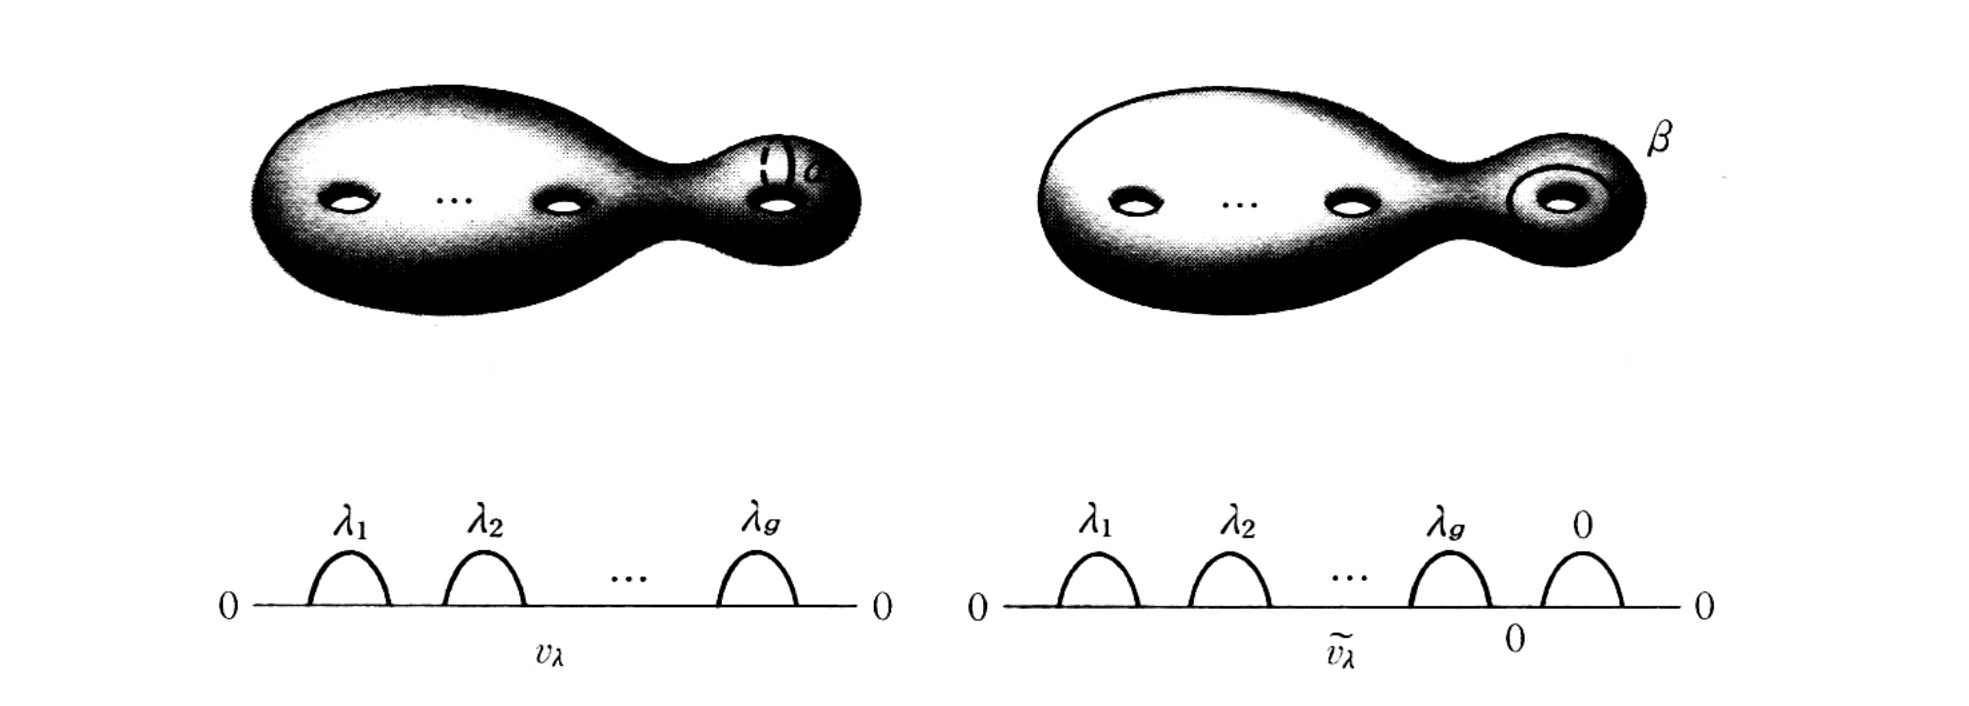
\includegraphics[width=0.96\textwidth]{figures/fig2.25.png}
  \figtitle{2.25}{原书无图注（原书 p.91）}
\end{figure}

给 $\Sigma$ 对应复线性空间，尝试构造 Atiyah 意义下的 2+1 维（拓扑场论）。这里，基本的配边是映射类群 $\cM_g$ 引起的柄体边界的粘合、添加柄的操作及其逆操作。$\Sigma$ 的亏格为 $g$ 时，作为 $\Sigma$ 对应的线性空间，取上面定义的
\[
  V_\Sigma=\bigoplus_{\mu_1,\mu_1^*,\dots,\mu_g,\mu_g^*\in P_+(k)}V_{\mu_1\mu_1^*\cdots\mu_g\mu_g^*}.
\]
关于映射类群 $\cM_g$ 的作用，已在命题 2.19 中说明。例如，对添加 1-柄的操作，用
\[
  \iota(v_\lambda)=\frac{1}{\sqrt{S_{00}}}\,\tilde v_\lambda
\]
定义 $\iota:V_{\partial H_g}\to V_{\partial H_{g+1}}$。这里，$\tilde v_\lambda$ 是如图2.25 所示，给 $v_\lambda$ 添加一个圈、并对添加的边赋权 $0$ 所得的 $V_{\partial H_{g+1}}$ 的元素。又对球面 $S^2$ 的生成元，用 $\beta(x)=\dfrac{x}{\sqrt{S_{00}}}$ 定义 $\beta:V_\phi\to V_{S^2}$。这里 $V_\phi=V_{S^2}=\C$。如此对配边对应线性映射，再作如下修正：公理 (A3) 在模去 $C$ 的适当幂次的意义下成立。这样就能构造出 2+1 维拓扑场论的例子。

% [Tutor Note: 添加 1-柄的算子 $\iota$ 前面的 $1/\sqrt{S_{00}}$ 与球面生成元 $\beta$ 的归一化是同一约定；漏掉这个因子会使公理 (A3) 的偏差不再是 $C$ 的幂次。]

这里不叙述细节，但上述构造可以推广到三维流形 $M$ 含链环 $L$ 的情形。链环各成分带有 framing 与定向，并被赋予 level $k$ 的最高权。

% [原文 p.92]
此时，作为切口出现的是图2.26 所示的闭曲面 $\Sigma$ 及其上有限个点 $p_1,\dots,p_n$；依链环成分的定向，这些点对应仿射 Lie 代数 $\hat\fg$ 的 level $k$ 的不可约表示或其对偶表示。这些权记作 $\lambda_1,\dots,\lambda_n$。同样把 $\Sigma$ 表示为图2.26 的图的正则邻域的边界，并令
\[
  V_{\Sigma,p,\lambda}=\bigoplus_{\mu_1,\mu_1^*,\dots,\mu_g,\mu_g^*\in P_+(k)}V_{\mu_1\mu_1^*\cdots\mu_g\mu_g^*\lambda_1\cdots\lambda_n}.
\]
用这个 $V_{\Sigma,p,\lambda}$，可以把命题 2.19 推广为 $\cM_{g,n}$ 的射影表示。这里，$\cM_{g,n}$ 是以 $n$ 个 $S^1$ 为边界的亏格 $g$ 曲面的映射类群。这种情形下也能对配边对应线性映射；特别地，当 $M=S^3$ 时，可以构造得使由这些线性映射的合成所定义的不变量 $Z(M,L;\lambda)$ 用 §2.2 定义的 $J(L;\lambda)$ 表为
\begin{equation}
  Z(M,L;\lambda)=S_{00}J(L;\lambda). \tag{2.30}
\end{equation}

特别地，考虑图2.26 所示给实心环体 $H$ 的中心线 $K$ 赋权 $\lambda$ 的情形。与边界 $T=\partial H$ 对应的是以 $v_\mu$（$0\le\mu\le k$）为基底的 $k+1$ 维线性空间 $V_T$。把由 $H,K,\lambda$ 确定的 $V_T$ 的向量记作 $\phi_\lambda$。由引理 2.9 关于平凡纽结的结果以及上面的 (2.30) 的条件，得
\[
  \langle Sv_0,\phi_\lambda\rangle=S_{\lambda0}.
\]
再结合式 (2.28) 所描述的 $SL_2(\Z)$ 在 $V_T$ 上的作用，可知 $\phi_\lambda=v_\lambda$。

下面从这个观点重新审视定理 2.16 中 $Z_k(M)$ 的定义式。当 $M$ 由沿 $S^3$ 中含 $m$ 个成分的链环 $L$ 的 Dehn 手术得到时，把链环 $L$ 的管状邻域的外部记作 $M_-$，把待粘合的实心环体的 $m$ 个并集记作 $M_+$，则 $Z_{M_+}=Z_T^{\otimes m}$。对 $M_-$ 确定向量 $Z(M_-)\in(Z_T^{\otimes m})^*$。把 Dehn 手术中出现的边界粘合映射记作 $f$，则 $f$ 在 $Z_T^{\otimes m}$ 上的作用表为
\[
  f v_{\mu_1}\otimes\cdots\otimes v_{\mu_m}=\sum_{\lambda}f_{\mu\lambda}v_{\lambda_1}\otimes\cdots\otimes v_{\lambda_m}.
\]
% [Tutor Note: (2.30) 只在 $M=S^3$ 时是构造中选定的归一化条件，并非对一般 $M$ 成立；一般 $M$ 的值须回到定理 2.16 的 Dehn 手术公式计算。]

% 块尾跨页句：f の Z_T^{⊗m} への作用を（p.93 冒頭の式で終わる）
% CHUNK ch02d DONE
